\section{Background}

%%In order to calculate the shutdown dose rate of a nuclear systems,
%%a nuclear inventory must be calculated

\subsection{Nuclear Inventory Analysis}
When a material is irradiated a variety of reactions can happen. These 
reactions may lead to production of radionuclides which can persist
after shutdown of the device. For Shutdown Dose Rate (SDR) Analysis, 
the nuclear inventory must be known
in order to quantify the photon emission density as a function of time.

The rate of change in the concentration of nuclide $i$ is given by the 
difference between the production rate and destruction rate of that nuclide.
The rate in which a nuclide undergoes transmutation to some other nuclide
is porportional to its concentration. 
\begin{equation}\label{rate_change_i}
  \frac{dN_{i}(t)}{dt} = \sum_{j} N_{j}P_{j \rightarrow i, total}
  - \sum_{j} N_{i}P_{i \rightarrow j, total}
\end{equation}
Transmutation can occur via a nuclear reaction or a decay. The total
proportionality constant is given by Equation \ref{total_p_const}.
\begin{equation}\label{total_p_const}
  P_{i \rightarrow j, total} = P_{i \rightarrow j, reaction } +
  P_{i \rightarrow j, decay}
\end{equation}
For the reaction process, the porpotionality constant is given by
Equation \ref{reaction_p_const}
\begin{equation}\label{reaction_p_const}
  P_{i \rightarrow j, reaction } =
  \int_{E_{n}} \sigma_{i \rightarrow j}(E_{n})
  \phi_{n}dE_{n}
\end{equation}
where $\sigma_{i \rightarrow j}(E_{n})$ is the microscopic cross
section for the reaction that transforms nuclide $i$ into $j$, and
 $\phi_{n}(E_{n})$ is the neutron flux for energy $E_{n}$.
For the decay process the proportionality constant is given by Equation
\ref{decay_p_const}

\begin{equation}\label{decay_p_const}
  P_{i \rightarrow j, decay} = \lambda_{i} b_{i \rightarrow j}
\end{equation}
where $\lambda_{i}$ is the decay constant and $b_{i \rightarrow j}$ is
the branching ratio.For entire network of nuclides,
Equation \ref{rate_change_i} can be expressed as
a systems of linear differential equations and is represented by Equation
\ref{rate_change_all}
\begin{equation}\label{rate_change_all}
  \frac{d\vec{N}}{dt} =\boldsymbol{A}  \vec{N}(t)
\end{equation}
where $\vec{N}(t)$ is the vector of all nuclide concentration and $boldsymbol{A}$
is the transfer matrix of production and desctruction rates. The solution to this
system of equations is given by Equation \ref{rate_change_sol}.
\begin{equation}\label{rate_change_sol}
  \vec{N} =\vec{N}_{o} e^{\boldsymbol{A}t}
\end{equation}


\subsection{Shutdown Dose Rate Analysis}

A primary method to investigate the SDR is known as the
Rigorous 2-Step (R2S) method. The R2S method consists of two transport steps
coupled by an activation step. 
The first transport calculation is performed, and the neutron flux tallied.
The neutron fluxes, and an irradiation scenerio are used in an activation
calculation using a dedicated nuclear iventory analysis code to give the 
photon density in the region as function of time. 
This photon density is then used as a source for photon transport,
where the SDR is tallied using a tally modified with flux-to-dose-rate
conversion factors.

\subsection{Shutdown Dose Rate for High Energy Systems}
One of the challeges presented when doing SDR analyses in high energy systems is the 
lack of nuclear cross-section tables in the energies higher than 20 MeV. 
The reaction proportionality constant, Equation \ref{reaction_p_const}
requires the neutron flux and the microscopic crossection of transmutting reaction. 
To gap this bridge, some activation codes accept productions and destruction rates
as their input. These production and destruction rates can be obtained from
physics models implemented in MCNP codes.
A radionuclide tally was implemented in MCNP to collect production and destruction
rates in a given geometric cell. The tally is a collision tally and
it collects reaction rates using the physics calculated
cross sections. A reaction rate for any reaction is given by Equation
\ref{reaction_rate_x}

\begin{equation}\label{reaction_rate_x}
  R_{x} = \Sigma_{x} \phi
\end{equation}
An estimate of the reaction rate is given by Equation \ref{reaction_rate_estimate}
\begin{equation}\label{reaction_rate_estimate}
  R_{x} = \frac{1}{W} \sum_{i \in A} w_{i}
\end{equation}
The flux can be estimated from a total reaction rate as seen in Equation
\ref{flux}
\begin{equation}\label{flux}
  \phi = \frac{1}{W} \sum_{i \in A} \frac{w_{i}}{\Sigma_{t}(E_{i})}
\end{equation}
Using Equation \ref{reaction_rate_x} and Equation \ref{flux}, we can get
the collision estimate of the reaction rate for reaction $x$
\begin{equation}\label{reaction_x_estimate}
  \phi = \frac{1}{W} \sum_{i \in A} \frac{w_{i} \Sigma_{x}(E_{i})}{\Sigma_{t}(E_{i})}
\end{equation}
The current SDR workflow is seen in Figure \ref{rnucs_r2s}
\begin{figure}[h!]
\begin{centering}
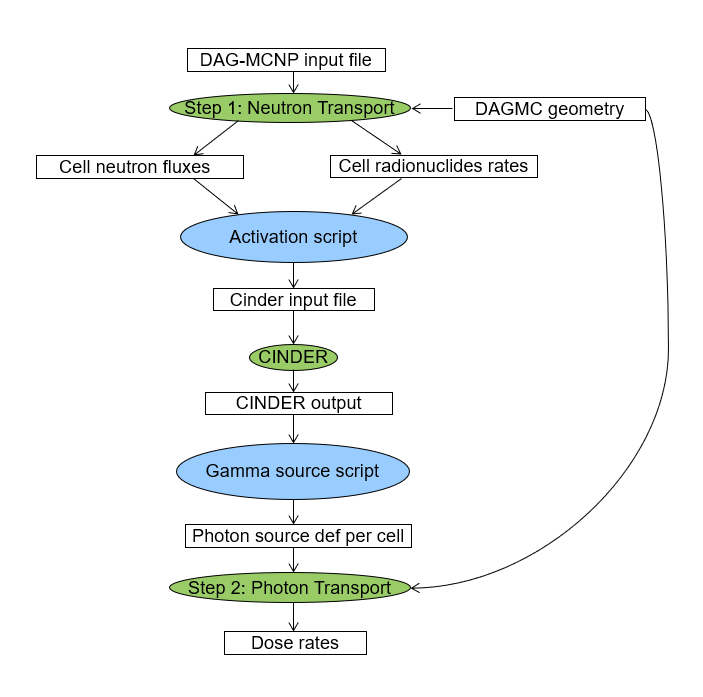
\includegraphics[scale=0.4]{../figs/rnucs_r2s.png}
\caption{Current shut down dose rate workflow for Accelerator systems as used by ORNL}
\label{rnucs_r2s}
\end{centering}
\end{figure}
\newpage
